\documentclass[11pt]{article}
\usepackage[margin=1.1in]{geometry}
\usepackage{amsmath,amssymb,amsthm}
\usepackage[round]{natbib}
\usepackage{xcolor}
\usepackage{hyperref}
\usepackage{booktabs}
\usepackage{pgfplots}
\pgfplotsset{compat=1.18}
\hypersetup{colorlinks=true,linkcolor=blue!50!black,citecolor=blue!50!black,urlcolor=blue!50!black}
\newtheorem{proposition}{Proposition}
\newtheorem{remark}{Remark}
\newtheorem{example}{Example}
\newcommand{\E}{\mathbb{E}}
\newcommand{\Var}{\mathrm{Var}}
\newcommand{\Cov}{\mathrm{Cov}}
\newcommand{\F}{\mathcal{F}}
\newcommand{\KL}{D_{\mathrm{KL}}}

\title{On the Importance of Evaluating Foundational Time-Series Models One Step Ahead in an Investment Context}
\author{Peter Cotton}
\date{November 2026}

\begin{document}
\maketitle

\begin{abstract}
Popular benchmarks for foundational time-series models pool forecast errors over long horizons. Under frictionless log utility, an investor who can trade every interval in a liquid market does not use those horizons: the optimal position depends only on the conditional distribution of the next return, and the investor's expected log-wealth regret from trading on a forecast is bounded by the forecast's excess expected log loss, its relative entropy from the truth. With transaction costs, in the quadratic model of G\^arleanu and Pedersen, later horizons enter through the expected-return path with weights that shift toward the next interval as costs fall. The one-step predictive is therefore the object to evaluate for that investor, its excess expected log loss controls the investor's regret without ranking imperfect forecasts' decisions, and a score pooled over horizons does not establish superiority for that decision. Two examples mark the limits: a model better at one step can be worse at twelve while iterating its own dynamics, and a forecast closer to the truth in relative entropy can induce the worse position. We recommend reporting one step ahead on its own and including an iterated one-step model among multi-step baselines.
\end{abstract}

\section{Setting}

A trader observes a liquid security at intervals (a day, an hour, a tick) and can trade once per interval at the quoted price. There is no market impact and, until Section~2.3, no transaction cost. Write $P_t$ for the price, $r_{t+1} = P_{t+1}/P_t - 1$ for the return over the next interval, $\F_t$ for the trader's information at $t$, and $x_t$ for the fraction of wealth held from $t$ to $t+1$. We call the interval between trades the \emph{decision interval}.

Does a forecast of $r_{t+2}, r_{t+3}, \dots$ change the choice of $x_t$? If it does not, a benchmark that scores such forecasts does not by itself establish performance for today's decision. The contribution is deliberately small. The sufficiency result is Mossin, Samuelson and Merton; the regret bound is Barron and Cover; the hedging demand is Merton; the cost-weighted aim portfolio is G\^arleanu and Pedersen; the comparison of direct and iterated forecasts is Marcellino, Stock and Watson. We line these up against the way multi-step forecasts of foundational time-series models are scored, keeping apart three questions: which distribution determines the optimal action, whether iterated or direct multi-step forecasts are better, and which loss evaluates a forecast for a stated decision.

\section{Which distribution determines the position}

\subsection{Log utility}

Wealth evolves as $W_{t+1} = W_t(1 + x_t r_{t+1})$ and the trader maximises $\E[\log W_T]$. Assume positive wealth, integrability of $\log(1 + x r_{t+1})$ on the feasible set, a feasible set of fractions that does not depend on wealth, and an exogenous opportunity process: a state $s_t$ adapted to $\F_t$ such that the conditional law of $(r_{t+1}, s_{t+1})$ given $\F_t$ depends on $\F_t$ only through $s_t$ and is unaffected by the trader's choices. The dynamic programme is
\begin{equation}
V_t(W_t, s_t) = \max_{x_t} \E\big[\,V_{t+1}(W_{t+1}, s_{t+1}) \,\big|\, s_t\big].
\label{eq:dp}
\end{equation}

\begin{proposition}[The next return's law is sufficient; \citealt{mossin1968}, \citealt{samuelson1969}, \citealt{merton1969}]
Under log utility and the assumptions above, $V_t(W, s) = \log W + g_t(s)$ for some $g_t$, and
\[
x_t^\ast = \arg\max_x \E\big[\log(1 + x r_{t+1}) \,\big|\, s_t\big].
\]
\end{proposition}
\begin{proof}
Induct backward from $V_T = \log W$. If $V_{t+1} = \log W + g_{t+1}(s)$ then
\[
\E[V_{t+1}(W_{t+1}, s_{t+1}) \mid s_t] = \log W_t + \E[\log(1 + x_t r_{t+1}) \mid s_t] + \E[g_{t+1}(s_{t+1}) \mid s_t],
\]
and because the opportunity process is exogenous only the middle term depends on $x_t$. Hence $g_t(s) = \max_x \E[\log(1 + x r_{t+1}) \mid s] + \E[g_{t+1}(s_{t+1}) \mid s]$.
\end{proof}

In English: the trader collects any predictability in later returns by trading when those intervals arrive, so today's position only has to be right about $r_{t+1}$. The state must be sufficient for the continuation value as well as for the next return's law. Holding the conditional law of $r_{t+1}$ and the feasible set fixed, predictability of $r_{t+12}$ from $\F_t$ changes $g_t$ and leaves the argmax alone; a signal about $r_{t+12}$ that also moves the conditional law of $r_{t+1}$ enters through that law. Kelly sizing \citep{kelly1956} is the same statement with $r$ a bet.

\subsection{Other utilities}

For $u(W) = W^{1-\gamma}/(1-\gamma)$ with $\gamma \ne 1$ the value function factorises as $V_t(W, s) = W^{1-\gamma} H_t(s)$. When returns are independent across intervals $H_{t+1}$ is constant and the problem is again one-period \citep{samuelson1969}. When returns are predictable, $H_{t+1}(s_{t+1})$ can covary with $r_{t+1}$ and \citet{merton1971,merton1973} obtain, in continuous time with one state variable,
\[
x_t^\ast = \frac{\mu_t - r^f}{\gamma \sigma_t^2} \;+\; \frac{\rho\, \sigma_{s}}{\sigma_t}\,\frac{-J_{Ws}}{W J_{WW}},
\]
where $\rho$ is the correlation between the return and the state innovation and $J$ is the value function. The second term is the hedging demand. It vanishes for $\gamma = 1$ and for $\rho = 0$, and it depends on how the opportunity set moves, through $J_{Ws}$.

\begin{remark}[Frequent trading does not shrink the hedging demand]
The decision interval and the remaining horizon $T - t$ are different quantities. Merton's formulation already allows continuous trading, and the hedging term is a function of the state dynamics with no factor in the trading interval. \citet{campbell1999} find in calibrated models with persistent expected returns that the hedging demand roughly doubles average stock demand for some investors, with a material loss from a myopic policy. The term can also be large relative to a myopic position that is itself near zero. The exact statement of this section is for log utility; for other utilities the frictionless position depends on the law of motion of the opportunity set.
\end{remark}

\subsection{Transaction costs}

Add a cost of trading and keep the trader once per interval in a liquid market. We switch to a tractable quadratic model and to one security. \citet{garleanu2013} study a trader holding $n_t$ shares with trading cost $\tfrac{1}{2}\lambda\sigma^2 (n_t - n_{t-1})^2$, mean-variance preferences with risk aversion $\gamma$ over the excess price change $\Delta P_{t+1}$ (net of financing; equivalently take the risk-free rate to be zero), variance $\sigma^2$, discount rate $\rho$, and expected excess price changes driven by mean-reverting factors. Write $m_h = \E_t[\mathrm{Markowitz}_{t+h}]$ with $\mathrm{Markowitz}_{t+h} = \E_{t+h}[\Delta P_{t+h+1}]/(\gamma\sigma^2)$, so that forecast lead $j = h + 1$. The optimal policy moves the holding a fixed fraction of the way toward an \emph{aim portfolio},
\begin{equation}
n_t = n_{t-1} + \frac{a}{\lambda}\,(\mathrm{aim}_t - n_{t-1}), \qquad
\mathrm{aim}_t = \sum_{h \ge 0} z(1-z)^h\, m_h,
\label{eq:gp}
\end{equation}
with
\[
a = \frac{-\big(\gamma(1-\rho) + \lambda\rho\big) + \sqrt{\big(\gamma(1-\rho) + \lambda\rho\big)^2 + 4\gamma\lambda(1-\rho)^2}}{2(1-\rho)}, \qquad z = \frac{\gamma}{\gamma + a}.
\]
The model's $n_t$ is a share holding and our $x_t$ a wealth fraction, so we quote \eqref{eq:gp} in its own units.

In English: the expected excess price change at every lead enters today's trade, weighted by how long the position will be carried, and the weights depend on the cost only through $\lambda/\gamma$. Within this model, holding the other parameters fixed, lowering the cost shifts the weight distribution toward the nearer leads. Figure~\ref{fig:weights} plots the weights by lead. Their half-life is $0.28$ leads at $\lambda/\gamma = 0.1$, $0.72$ at $1$, $2.2$ at $10$ and $6.9$ at $100$; the mass beyond lead twelve is $0.001$ percent at $\lambda/\gamma = 1$, $2.3$ percent at $10$ and $30$ percent at $100$. The figure is a sensitivity analysis; we do not map a particular security and interval to a value of $\lambda/\gamma$.

Concentrated weights bound the absolute contribution of later leads and nothing more. Since $\mathrm{aim}_t - m_0 = \sum_{h \ge 1} z(1-z)^h (m_h - m_0)$, a bound $\sup_{h \ge 1} |m_h - m_0| \le C$ gives $|\mathrm{aim}_t - m_0| \le C(1-z)$. When $m_0$ is near zero the relative error is not small: two predictive factors can cancel today and decay at different rates, leaving the whole aim to later leads. Other objectives need not admit fixed horizon weights at all; with proportional costs, constraints or nonlinear utility the policy can involve state-dependent trading regions.

\begin{figure}[t!]
\centering
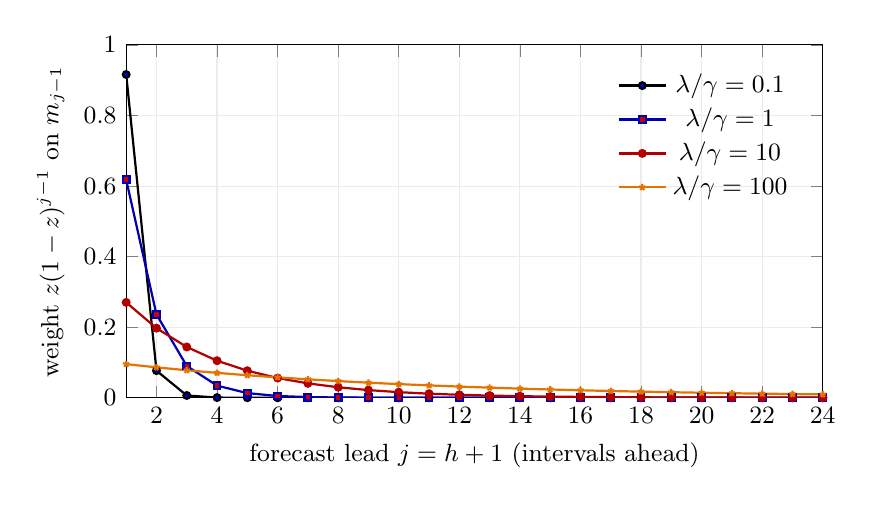
\begin{tikzpicture}
\pgfmathsetmacro{\rhoo}{0.0004}
\pgfmathsetmacro{\za}{1/(1+(-(1*(1-\rhoo)+0.1*\rhoo)+sqrt((1*(1-\rhoo)+0.1*\rhoo)^2+4*1*0.1*(1-\rhoo)^2))/(2*(1-\rhoo)))}
\pgfmathsetmacro{\zb}{1/(1+(-(1*(1-\rhoo)+1*\rhoo)+sqrt((1*(1-\rhoo)+1*\rhoo)^2+4*1*1*(1-\rhoo)^2))/(2*(1-\rhoo)))}
\pgfmathsetmacro{\zc}{1/(1+(-(1*(1-\rhoo)+10*\rhoo)+sqrt((1*(1-\rhoo)+10*\rhoo)^2+4*1*10*(1-\rhoo)^2))/(2*(1-\rhoo)))}
\pgfmathsetmacro{\zd}{1/(1+(-(1*(1-\rhoo)+100*\rhoo)+sqrt((1*(1-\rhoo)+100*\rhoo)^2+4*1*100*(1-\rhoo)^2))/(2*(1-\rhoo)))}
\begin{axis}[width=0.86\textwidth,height=0.5\textwidth,
  xlabel={forecast lead $j = h+1$ (intervals ahead)}, ylabel={weight $z(1-z)^{j-1}$ on $m_{j-1}$},
  xmin=1, xmax=24, ymin=0, ymax=1, samples at={1,...,24},
  legend style={draw=none, fill=none, at={(0.97,0.95)}, anchor=north east, font=\small},
  grid=major, grid style={draw=black!8}, tick label style={font=\small}, label style={font=\small},
  every axis plot/.append style={thick, mark=*, mark size=1.2pt}]
\addplot+[black] {\za*(1-\za)^(x-1)}; \addlegendentry{$\lambda/\gamma = 0.1$}
\addplot+[blue!70!black] {\zb*(1-\zb)^(x-1)}; \addlegendentry{$\lambda/\gamma = 1$}
\addplot+[red!70!black] {\zc*(1-\zc)^(x-1)}; \addlegendentry{$\lambda/\gamma = 10$}
\addplot+[orange!90!black] {\zd*(1-\zd)^(x-1)}; \addlegendentry{$\lambda/\gamma = 100$}
\end{axis}
\end{tikzpicture}
\caption{Weight of each forecast lead's expected excess price change in the aim portfolio of equation~\eqref{eq:gp}, per-interval discount rate $\rho = 0.0004$ (about ten percent a year at daily intervals). Lower cost puts the weight on the first lead; at $\lambda/\gamma = 1$ the first two leads carry 85 percent of it.}
\label{fig:weights}
\end{figure}

\subsection{Excluded constraints and payoffs}

A lock-up or a monthly mandate fixes a holding period, and the decision then depends on the cumulative return $R_{t,k} = \prod_{j=1}^{k}(1 + r_{t+j}) - 1$; a position too large to unwind in one interval imposes a liquidation schedule instead, which is a path problem. A futures expiry fixes neither; the position can be closed before it. Horizon risk limits and derivatives are compatible with trading once per interval and attach future-dependent valuation or constraints to today's choice; drawdown and barrier contracts depend on path functionals rather than on cumulative-return marginals. We exclude these constraints and payoffs.

\section{Direct and iterated multi-step forecasts}

\subsection{What an iterated one-step model requires}

The joint law of the next $k$ returns given $\F_t$ factorises as
\[
p(r_{t+1}, \dots, r_{t+k} \mid \F_t) = \prod_{h=1}^{k} p\big(r_{t+h} \,\big|\, \F_t, r_{t+1}, \dots, r_{t+h-1}\big).
\]
A one-step model supplies the first factor at the current state. To supply the rest it must be a generative model with specified state dynamics: it must say how its state moves when a return is appended, and it must model, or integrate out, any exogenous information that arrives between $t$ and $t+h$. A one-step predictive at the present state and a complete transition model are different objects. A forecaster can score well when updated with realised observations and badly when iterated on its own simulated ones.

The chain rule also removes an apparent dichotomy. Any joint law admits an autoregressive factorisation, including a law fitted jointly across horizons; and separately fitted horizon marginals do not by themselves specify a joint law.

\subsection{No ordering across horizons}

A correct transition model gives correct forecasts at every horizon. Among imperfect models no ordering follows, with or without Markov structure in the truth.

\begin{example}[Better at one step, worse at twelve]
Let returns take the values $\pm a$ as the states of a two-state chain with transition matrix $M(p)$, $p$ the probability of staying, so that $\Pr(X_{t+h} = X_t) = \tfrac{1}{2}\big(1 + (2p-1)^h\big)$. Let the truth be $M(0.9)$, model $A$ be $M(0.8)$ and model $B$ be $M(0.1)$, each iterating its own matrix. At one step $A$ is far better: its excess expected log loss is about $0.037$ against $1.758$ for $B$. At twelve steps $B$ is exactly right, because $M(0.1)^{12} = M(0.9)^{12}$.
\end{example}

Whether a direct $h$-step forecast beats an iterated one-step model is therefore a question about estimation efficiency and misspecification. \citet{marcellino2006} treat it as such and find no universal winner. It has to be measured.

\subsection{Three targets}

Three objects need separate names: a single interval's return $r_{t+h}$, the cumulative return $R_{t,h}$, and the path $(r_{t+1}, \dots, r_{t+h})$. A model that is better at $r_{t+12}$ is not thereby better for a twelve-interval holding decision, which depends on $R_{t,12}$. Good cumulative-return marginals at several horizons do not establish that a model captures path dependence; different joint laws share those marginals and imply different drawdown risks.

\section{Forecast quality and decision quality}

Proposition~1 names the distribution that determines the optimal action. Two further facts fix what a score of that distribution does and does not tell the trader.

\begin{proposition}[Relative entropy bounds the log-utility regret; \citealt{barron1988}]
Let $P$ be the true conditional law of $r$ and $Q$ a forecast, let the feasible set of fractions be convex and common to both, with $1 + xr > 0$ on it, and let the expectations below be finite. With $x_P \in \arg\max_x \E_P \log(1 + xr)$ and $x_Q \in \arg\max_x \E_Q \log(1 + xr)$,
\[
0 \le \E_P\!\left[\log \frac{1 + x_P r}{1 + x_Q r}\right] \le \KL(P \,\|\, Q).
\]
\end{proposition}
\begin{proof}
Optimality of $x_Q$ under $Q$ over a convex set gives the first-order condition $\E_Q\big[(1 + x r)/(1 + x_Q r)\big] \le 1$ for every feasible $x$, in particular for $x_P$. Then, writing $p$ and $q$ for the densities,
\[
\E_P\!\left[\log \frac{1 + x_P r}{1 + x_Q r}\right]
= \KL(P\|Q) + \E_P\!\left[\log\Big(\frac{q}{p}\,\frac{1 + x_P r}{1 + x_Q r}\Big)\right]
\le \KL(P\|Q) + \log \E_Q\!\left[\frac{1 + x_P r}{1 + x_Q r}\right] \le \KL(P\|Q),
\]
by Jensen's inequality and the first-order condition. The lower bound is optimality of $x_P$ under $P$.
\end{proof}

In English: the expected log-wealth lost by trading on a forecast is at most the forecast's excess expected log loss. A smaller excess loss tightens the trader's guarantee; a realised log score on a sample estimates it with error. It does not rank decisions.

\begin{example}[The better forecast induces the worse position]
Let returns take the values $\{-0.2, 0, 0.2\}$ with truth $(0.20, 0.50, 0.30)$, forecast $A = (0.21, 0.50, 0.29)$ and forecast $B = (0.32, 0.20, 0.48)$. The log-optimal fraction is $x^\ast(q) = \big(q(0.2) - q(-0.2)\big)/\big(0.2\,[q(0.2) + q(-0.2)]\big)$, which equals $1.00$ under the truth, $0.80$ under $A$ and $1.00$ under $B$, while $\KL(P\|A) \approx 0.0004$ and $\KL(P\|B) \approx 0.223$. Proposition~2 bounds $A$'s regret by $0.0004$ and $B$'s by $0.223$; $B$'s regret is zero.
\end{example}

The bound is specific to logarithmic scoring under these conditions and says nothing about other proper scores. The same distinction applies to a model $B$ that is the better forecaster at twelve steps while $A$ is better at one. Let $\mathcal{I}_A \subseteq \F_t$ be the inputs model $A$ uses. $B$'s output is $\F_t$-measurable, so it adds nothing to the oracle law $p(r_{t+1} \mid \F_t)$; it can still improve $A$, and conditioning $A$ on it has value exactly when the conditional law of $r_{t+1}$ given $\mathcal{I}_A$ and $B$'s output differs from the law given $\mathcal{I}_A$ alone. Mixture weights chosen by predictive log score are likewise a forecasting choice; a trader with a stated objective would in general choose others.

\section{Testing a one-step model against a multi-step one}

Three constructions use a one-step model $A$ with a multi-step model $B$ and can be tested for improvement without retraining either. Each is evaluated at the information set it uses.

\emph{A portfolio per horizon.} At each $h$, mix the two predictive marginals with weights that follow realised score at that horizon. This needs $A$'s marginal at every horizon, so $A$ must be iterated as a generative model (Section~3.1) or supplied with separate horizon forecasts; we iterate. The weights report where each model is better. The mixed marginals do not specify a joint path law, so the construction is evaluated on marginals unless a dependence structure is added.

\emph{Marginal replacement.} If $B$ emits sample paths from a joint law $p_B$ with first-step marginal $p_{B,1}$, give each path the importance weight $p_A(x_1)/p_{B,1}(x_1)$. The weighted law is
\[
q(x_{1:H}) = p_B(x_{1:H})\,\frac{p_A(x_1)}{p_{B,1}(x_1)} = p_A(x_1)\, p_B(x_{2:H} \mid x_1),
\]
$A$'s first-step marginal with $B$'s conditional law of the rest of the path given the first observation. It preserves that conditional law and need not preserve $B$'s copula or unconditional correlations. Under the true law $P$, when the expectations are well defined and finite,
\[
\E_P\big[\log q(X_{1:H}) - \log p_B(X_{1:H})\big] = \E_P\big[\log p_A(X_1) - \log p_{B,1}(X_1)\big],
\]
so the path log score improves by exactly the first-step improvement, when there is one. The identity says nothing about later marginals, cumulative-return scores or utility. The construction needs $p_{B,1}$ to be positive wherever $p_A$ is, evaluable first-step densities, and control of weight degeneracy; it is made at time $t$.

\emph{Revision by the one-step innovation.} A stale $h$-step forecast made at $t$ can be revised, once $r_{t+1}$ is seen, by the regression of its error on the surprise $r_{t+1} - \E^A_t[r_{t+1}]$. The revised forecast is an object of time $t+1$ and is compared with competitors that hold the same information at $t+1$ for the same target date. Rerunning $B$ at $t+1$ makes the revision redundant only if the rerun absorbs the new observation adequately.

The experiment is then: $B$ alone, $A$ iterated alone, and each construction, at identical origins and information sets, scored on $r_{t+h}$ per horizon, with cumulative-return and path-functional scores for the constructions that supply a joint law.

\section{Benchmarks of foundational time-series models}

GIFT-Eval \citep{aksu2024gifteval} evaluates on non-overlapping rolling windows in the test portion of each series, one window in some configurations and several in others; averages a quantile loss over nine levels and over every position of a window that spans several seasonal periods; normalises each metric against a seasonal naive per configuration; and aggregates across configurations by geometric mean, with average ranks alongside. The suites surveyed in \citet{cotton2026stronger} share the pooling of positions within a window.

For the once-per-interval trader in a liquid market four statements hold.

\begin{enumerate}
\item One step ahead at the decision interval should be reported on its own. For the log-utility trader the one-step predictive is the only input to the decision, and by Proposition~2 its excess expected log loss bounds the trader's regret. The decision interval belongs to the trader; a daily dataset scored at $h = 1$ speaks to a trader who trades daily.
\item An equal-weight average over horizons has economic readings. An unnormalised sum of pinball losses is the objective of a collection of quantile decisions with additive asymmetric costs at different dates, and a uniformly distributed compulsory liquidation date gives an equal-weight average of horizon utilities. Neither reading is this trader's, so a pooled headline does not establish superiority for this trader.
\item The multi-step baseline should include an iterated one-step model with specified state dynamics, compared at identical origins and information on $r_{t+h}$, and on $R_{t,h}$ and path functionals where the models supply a joint law. Section~3.2 is the reason the comparison has to be run.
\item Where a decision is named, its regret belongs next to the score. Proposition~2 bounds it for the log-utility trader; Section~2.3 shows that the aim portfolio's weights do not convert into a per-horizon score.
\end{enumerate}

This is why the \texttt{skaters} package scores \texttt{laplace(k=1)} and why its comparison with foundational time-series models on \url{https://foundationalprediction.com} is made one step ahead and never pooled across horizons. The package's twelve-step limit and its decimated multi-scale fans are engineering choices documented in the package; nothing here derives them. We leave to future work the experiment of Section~5 on the canonical panel, with predictive scores next to the regret of a stated trading rule.

\section*{Disclosure}

Drafting was assisted by Anthropic's Claude. The two examples, the marginal-replacement identity and the pointer to the Barron--Cover bound came from reviews produced by OpenAI's ChatGPT. The author directed and checked the work.

\bibliographystyle{plainnat}
\bibliography{horizon-note}
\end{document}
